%LaTeX reported generated by EES
\documentclass[10pt,fleqn]{article}
%%%%%%%%%%%%%%%%%%%%%%%%%%%%% Define Article %%%%%%%%%%%%%%%%%%%%%%%%%%%%%%%%%%
%%%%%%%%%%%%%%%%%%%%%%%%%%%%%%%%%%%%%%%%%%%%%%%%%%%%%%%%%%%%%%%%%%%%%%%%%%%%%%%

%%%%%%%%%%%%%%%%%%%%%%%%%%%%% Using Packages %%%%%%%%%%%%%%%%%%%%%%%%%%%%%%%%%%
\usepackage{float}
% \usepackage[letterpaper,portrait]{geometry}
\usepackage{graphicx}
\usepackage{anysize}
\usepackage{lipsum}
\usepackage{amsmath,amssymb,amsthm}
\usepackage[utf8]{inputenc}
\usepackage{multirow}
\usepackage{csquotes}
\usepackage[spanish]{babel}
\usepackage{apacite}
\usepackage{multicol}
\usepackage{parskip}
\usepackage{setspace}
\usepackage{empheq}
\usepackage{mdframed}
\usepackage{booktabs}
\usepackage{lipsum}
\usepackage{graphicx}
\usepackage{color}
\usepackage{psfrag}
\usepackage{pgfplots}
\usepackage{bm}
\usepackage{tocloft}
\usepackage{lscape}
\usepackage{adjustbox}
\usepackage[margin=2.54cm]{geometry}
\setlength{\tabcolsep}{1.505625pt}
\renewcommand{\arraystretch}{1.2}
%%%%%%%%%%%%%%%%%%%%%%%%%%%%%%%%%%%%%%%%%%%%%%%%%%%%%%%%%%%%%%%%%%%%%%%%%%%%%%%

% Other Settings

%%%%%%%%%%%%%%%%%%%%%%%%%% Page Setting %%%%%%%%%%%%%%%%%%%%%%%%%%%%%%%%%%%%%%%
\geometry{letterpaper, margin=2.54cm}

%%%%%%%%%%%%%%%%%%%%%%%%%% Define some useful colors %%%%%%%%%%%%%%%%%%%%%%%%%%
\definecolor{ocre}{RGB}{243,102,25}
\definecolor{mygray}{RGB}{243,243,244}
\definecolor{deepGreen}{RGB}{26,111,0}
\definecolor{shallowGreen}{RGB}{235,255,255}
\definecolor{deepBlue}{RGB}{61,124,222}
\definecolor{shallowBlue}{RGB}{235,249,255}
%%%%%%%%%%%%%%%%%%%%%%%%%%%%%%%%%%%%%%%%%%%%%%%%%%%%%%%%%%%%%%%%%%%%%%%%%%%%%%%

%%%%%%%%%%%%%%%%%%%%%%%%%% Define an orangebox command %%%%%%%%%%%%%%%%%%%%%%%%
\newcommand\orangebox[1]{\fcolorbox{ocre}{mygray}{\hspace{1em}#1\hspace{1em}}}
%%%%%%%%%%%%%%%%%%%%%%%%%%%%%%%%%%%%%%%%%%%%%%%%%%%%%%%%%%%%%%%%%%%%%%%%%%%%%%%

%%%%%%%%%%%%%%%%%%%%%%%%%%%% English Environments %%%%%%%%%%%%%%%%%%%%%%%%%%%%%
\newtheoremstyle{mytheoremstyle}{3pt}{3pt}{\normalfont}{0cm}{\rmfamily\bfseries}{}{1em}{{\color{black}\thmname{#1}~\thmnumber{#2}}\thmnote{\,--\,#3}}
\newtheoremstyle{myproblemstyle}{3pt}{3pt}{\normalfont}{0cm}{\rmfamily\bfseries}{}{1em}{{\color{black}\thmname{#1}~\thmnumber{#2}}\thmnote{\,--\,#3}}
\theoremstyle{mytheoremstyle}
\newmdtheoremenv[linewidth=1pt,backgroundcolor=shallowGreen,linecolor=deepGreen,leftmargin=0pt,innerleftmargin=20pt,innerrightmargin=20pt,]{theorem}{Theorem}[section]
\theoremstyle{mytheoremstyle}
\newmdtheoremenv[linewidth=1pt,backgroundcolor=shallowBlue,linecolor=deepBlue,leftmargin=0pt,innerleftmargin=20pt,innerrightmargin=20pt,]{definition}{Definition}[section]
\theoremstyle{myproblemstyle}
\newmdtheoremenv[linecolor=black,leftmargin=0pt,innerleftmargin=10pt,innerrightmargin=10pt,]{problem}{Problem}[section]
%%%%%%%%%%%%%%%%%%%%%%%%%%%%%%%%%%%%%%%%%%%%%%%%%%%%%%%%%%%%%%%%%%%%%%%%%%%%%%%

%%%%%%%%%%%%%%%%%%%%%%%%%%%%%%% Plotting Settings %%%%%%%%%%%%%%%%%%%%%%%%%%%%%
\usepgfplotslibrary{colorbrewer}
\pgfplotsset{width=8cm,compat=1.9}
%%%%%%%%%%%%%%%%%%%%%%%%%%%%%%%%%%%%%%%%%%%%%%%%%%%%%%%%%%%%%%%%%%%%%%%%%%%%%%%

%%%%%%%%%%%%%%%%%%%%%%%%%%%%%%% Title & Author %%%%%%%%%%%%%%%%%%%%%%%%%%%%%%%%
\author{Gustavo Vergara}
\mathindent 0.0in
\usepackage[ansinew]{inputenc}
\usepackage{graphicx}
\usepackage{color}
\definecolor{silver}{rgb}{0.75,0.75,0.75}
\definecolor{gray}{rgb}{0.5,0.5,0.5}
\definecolor{aqua}{rgb}{0.5,1,1}
\definecolor{navy}{rgb}{0.0,0.0,0.5}
\definecolor{orange}{rgb}{1.0,0.5,0.0}
\definecolor{teal}{rgb}{0.25,0.5,0.5}
\definecolor{olive}{rgb}{0.5,0.5,0.0}
\definecolor{purple}{rgb}{0.5,0.0,0.5}
\definecolor{brown}{rgb}{0.5,0.25,0.0}
\definecolor{fuchsia}{rgb}{1.0,0.5,1.0}
\definecolor{buff}{rgb}{1.0,0.94,0.80}
\definecolor{lime}{rgb}{0.5,1.0,0.0}
\setlength{\headsep}{-0.6in}
\setlength{\textheight}{9in}
\setlength{\footskip}{1.0 in}
\setlength{\oddsidemargin}{-0.2in}
\setlength{\evensidemargin}{-0.2in}
\setlength{\textwidth}{6.8in}
\usepackage{longtable}
\newcommand{\abs}[1]{\left|#1\right|}
\newcommand{\F}[1]{\mbox{$#1$}}
\newcommand{\K}[1]{\mbox{\sf#1\ \ \mit}}
\newcommand{\KS}[1]{\mbox{\sf\ \ #1\ \ \mit}}
\newcommand{\SC}[1]{\mbox{`#1'}\  }
\newcommand{\V}[1]{\mbox{$ #1 $}}
\newcommand{\I}{\mbox{\hspace{0.20in}}}
\newcommand{\temperature}{\mathrm{T}}
\newcommand{\pressure}{\mathrm{P}}
\newcommand{\volume}{\mathrm{v}}
\newcommand{\density}{\mathrm{\rho}}
\newcommand{\intenergy}{\mathrm{u}}
\newcommand{\enthalpy}{\mathrm{h}}
\newcommand{\entropy}{\mathrm{s}}
\newcommand{\molarmass}{\mathrm{MW}}
\newcommand{\enthalpyfusion}{\mathrm{\Delta h_{fusion}}}
\newcommand{\quality}{\mathrm{x}}
\newcommand{\viscosity}{\mathrm{\mu}}
\newcommand{\conductivity}{\mathrm{k}}
\newcommand{\prandtl}{\mathrm{P_r}}
\newcommand{\cp}{\mathrm{c_p}}
\newcommand{\cv}{\mathrm{c_v}}
\newcommand{\specheat}{\mathrm{c_p}}
\newcommand{\soundspeed}{\mathrm{c}}
\newcommand{\wetbulb}{\mathrm{wb}}
\newcommand{\humrat}{\mathrm{\omega}}
\newcommand{\acentricfactor}{\mathrm{\omega}}
\newcommand{\relhum}{\mathrm{\phi}}
\newcommand{\dewpoint}{\mathrm{DP}}
\newcommand{\volexpcoef}{\mathrm{\beta}}
\newcommand{\compressibilityfactor}{\mathrm{Z}}
\newcommand{\surfacetension}{\mathrm{\gamma}}
\newcommand{\tcrit}{\mathrm{T_{crit}}}
\newcommand{\pcrit}{\mathrm{P_{crit}}}
\newcommand{\vcrit}{\mathrm{v_{crit}}}
\newcommand{\ttriple}{\mathrm{T_{triple}}}
\newcommand{\fugacity}{\mathrm{fugacity}}
\newcommand{\tsat}{\mathrm{T_{sat}}}
\newcommand{\psat}{\mathrm{P_{sat}}}
\newcommand{\eklj}{\mathrm{ek_{LJ}}}
\newcommand{\sigmalj}{\mathrm{\sigma_{LJ}}}
\begin{document}
\begin{titlepage}
	\centering
	\vspace{2.5cm}
	{\scshape \Large TALLER DE MÁQUINAS TÉRMICAS\par}
	\vspace{5cm}
	\textbf\large\scshape{\par}
	\vspace{0.5cm}
	{\Large Vergara Pareja Gustavo\par}
    {\Large Martínez Causil Carlos Alberto\par}
    {\Large Soto Suárez Iván Esteban\par}
    {\Large Quintero Martínez Jean Paul\par}
	\vspace{5cm}
	{\scshape\Large Bernardo J. Luján E. \par}
	\vspace{0.3cm}
	{\scshape\Large Máquinas Térmicas - G2IM \par}
	\vspace{0.3cm}
	{\scshape\Large Universidad de Córdoba\par}
	\vspace{0.3cm}
	{\Large 13 de Noviembre de 2024 \par}
\end{titlepage}
%\tableofcontents
\begin{center}
\bf \mbox{Ciclo de potencia a vapor}
\vspace{0.2 in}
\end{center}
\subsection*{Equations}

\vspace{0.10in}
\noindent
{\color{blue} \rm Turbina}
\begin{equation}
\label{EES Eqn:1}
\K{procedure} \F{Analisis_{Turbina}}{ \left( h_{in},\ s_{in},\ P_{in},\ P_{out},\ \eta_{t}:h_{out},\ s_{out},\ T_{out} \right) } 
\end{equation}
\begin{equation}
\I \label{EES Eqn:2}
h_{s,out} = \enthalpy \left(\F{Water},\mbox{\ s}=s_{in},\mbox{\ P}=P_{out} \right)  
\end{equation}
\begin{equation}
\I \label{EES Eqn:3}
h_{out} = h_{in}-\eta_{t}\cdot  \left( h_{in}-h_{s,out} \right)  
\end{equation}
\begin{equation}
\I \label{EES Eqn:4}
s_{out} = \entropy \left(\F{Water},\mbox{\ P}=P_{out},\mbox{\ h}=h_{out} \right)  
\end{equation}
\begin{equation}
\I \label{EES Eqn:5}
T_{out} = \temperature \left(\F{Water},\mbox{\ P}=P_{out},\mbox{\ h}=h_{out} \right)  
\end{equation}
\begin{equation}
\label{EES Eqn:6}
\K{end} 
\end{equation}

\vspace{0.10in}
\noindent
\vspace{0.1 in}
{\color{blue} \rm Bomba}
\begin{equation}
\label{EES Eqn:7}
\K{procedure} \F{Analisis_{Bomba}}{ \left( h_{in},\ s_{in},\ P_{in},\ P_{out},\ \eta_{b}:h_{out},\ s_{out},\ T_{out} \right) } 
\end{equation}
\begin{equation}
\I \label{EES Eqn:8}
h_{s,out} = \enthalpy \left(\F{Water},\mbox{\ s}=s_{in},\mbox{\ P}=P_{out} \right)  
\end{equation}
\begin{equation}
\I \label{EES Eqn:9}
h_{out} =  \left( \frac {h_{s,out}-h_{in}}{ \eta_{b} } \right) +h_{in} 
\end{equation}
\begin{equation}
\I \label{EES Eqn:10}
s_{out} = \entropy \left(\F{Water},\mbox{\ P}=P_{out},\mbox{\ h}=h_{out} \right)  
\end{equation}
\begin{equation}
\I \label{EES Eqn:11}
T_{out} = \temperature \left(\F{Water},\mbox{\ P}=P_{out},\mbox{\ h}=h_{out} \right)  
\end{equation}
\begin{equation}
\label{EES Eqn:12}
\K{end} 
\end{equation}

\vspace{0.10in}
\noindent
\vspace{0.1 in}
{\color{red} \bf Condiciones de operaci�n$_{,,,,,,,,,,,,,,,,,,,,,,,,,,,,,,,,,,,,,,,,,,,,}$}
\begin{equation}
\label{EES Eqn:13}
\dot {m}_{b} = 2.5  \   \left[ \rm kg/s \right] 
\end{equation}
{\color{blue} \rm}
\begin{equation}
\label{EES Eqn:14}
P_{b} = 10\cdot \rm { \left|1\ {\rm1} \right|} 
\end{equation}
\begin{equation}
\label{EES Eqn:15}
T_{hf,in} = 450 
\end{equation}

\vspace{0.10in}
\noindent
{\color{blue} \rm Presiones de  extraccion$<$$<$$<$$<$$<$$<$$<$$<$$<$$<$$<$$<$$<$$<$$<$$<$$<$$<$$<$$<$$<$$<$$<$}
\begin{equation}
\label{EES Eqn:16}
P_{ext,1} = 1.1\times 10^{3}  \   \left[ \rm kPa \right] 
\end{equation}
{\color{blue} \rm}
\begin{equation}
\label{EES Eqn:17}
P_{ext,2} = 0.25\times 10^{3}  \   \left[ \rm kPa \right] 
\end{equation}
{\color{blue} \rm}
\begin{equation}
\label{EES Eqn:18}
P_{ext,3} = 0.1\times 10^{3}  \   \left[ \rm kPa \right] 
\end{equation}
{\color{blue} \rm}

\vspace{0.10in}
\noindent
{\color{blue} \rm Eficiencias}
\begin{equation}
\label{EES Eqn:19}
\eta_{T,1}=0.87 
\end{equation}
\begin{equation}
\label{EES Eqn:20}
\eta_{T,2}=0.90 
\end{equation}
\begin{equation}
\label{EES Eqn:21}
\eta_{T,3}=0.92 
\end{equation}
\begin{equation}
\label{EES Eqn:22}
\eta_{T,4}=0.93 
\end{equation}
\begin{equation}
\label{EES Eqn:23}
\eta_{P,1}=0.65 
\end{equation}
\begin{equation}
\label{EES Eqn:24}
\eta_{P,2}=0.67 
\end{equation}
\begin{equation}
\label{EES Eqn:25}
\eta_{P,3}=0.69 
\end{equation}
\begin{equation}
\label{EES Eqn:26}
{\Delta T}_{b} = 15   \   \left[ \rm C \right] 
\end{equation}
{\color{blue} \rm}
\begin{equation}
\label{EES Eqn:27}
{\Delta T}_{rh} = 10   \   \left[ \rm C \right] 
\end{equation}
{\color{blue} \rm}
\begin{equation}
\label{EES Eqn:28}
{\Delta T}_{cond} = 5   \   \left[ \rm C \right] 
\end{equation}
{\color{blue} \rm}
\begin{equation}
\label{EES Eqn:29}
{\Delta T}_{CAA,C} = 2   \   \left[ \rm C \right] 
\end{equation}
{\color{blue} \rm}
\begin{equation}
\label{EES Eqn:30}
T_{c} = 30   \   \left[ \rm C \right] 
\end{equation}
{\color{blue} \rm}

\vspace{0.10in}
\noindent
{\color{red} \bf Estados$_{,,,,,,,,,,,,,,,,,,,,,,,,,,,,,,,,,,,,,,,,,,,,,,,,,,,,}$}

\vspace{0.10in}
\noindent
{\color{blue} \rm Estado 1}
\begin{equation}
\label{EES Eqn:31}
P_{1}=P_{b} 
\end{equation}
\begin{equation}
\label{EES Eqn:32}
T_{1}=\temperature \left(\F{Water},\mbox{\ P}=P_{1},\mbox{\ h}=h_{1} \right)  
\end{equation}
\begin{equation}
\label{EES Eqn:33}
s_{1}=\entropy \left(\F{Water},\mbox{\ h}=h_{1},\mbox{\ P}=P_{1} \right)  
\end{equation}

\vspace{0.10in}
\noindent
{\color{blue} \rm Estado 2}
\begin{equation}
\label{EES Eqn:34}
P_{2}=P_{1} 
\end{equation}
\begin{equation}
\label{EES Eqn:35}
T_{2}=T_{hf,in}-{\Delta T}_{b} 
\end{equation}
\begin{equation}
\label{EES Eqn:36}
h_{2}=\enthalpy \left(\F{Water},\mbox{\ T}=T_{2},\mbox{\ P}=P_{2} \right)  
\end{equation}
\begin{equation}
\label{EES Eqn:37}
s_{2}=\entropy \left(\F{Water},\mbox{\ T}=T_{2},\mbox{\ P}=P_{2} \right)  
\end{equation}

\vspace{0.10in}
\noindent
{\color{blue} \rm Estado 3}
\begin{equation}
\label{EES Eqn:38}
P_{3}=P_{ext,1} 
\end{equation}
\begin{equation}
\label{EES Eqn:39}
\K{call} \F{Analisis_{Turbina}}{ \left( h_{2},\ s_{2},\ P_{2},\ P_{3},\ \eta_{T,1}:h_{3},\ s_{3},\ T_{3} \right) } 
\end{equation}

\vspace{0.10in}
\noindent
{\color{blue} \rm Estado 4}
\begin{equation}
\label{EES Eqn:40}
P_{4}=P_{ext,2} 
\end{equation}
\begin{equation}
\label{EES Eqn:41}
\K{call} \F{Analisis_{Turbina}}{ \left( h_{3},\ s_{3},\ P_{3},\ P_{4},\ \eta_{T,2}:h_{4},\ s_{4},\ T_{4} \right) } 
\end{equation}

\vspace{0.10in}
\noindent
{\color{blue} \rm Estado 5}
\begin{equation}
\label{EES Eqn:42}
P_{5}=P_{4} 
\end{equation}
\begin{equation}
\label{EES Eqn:43}
T_{5}=T_{hf,in}-{\Delta T}_{rh} 
\end{equation}
\begin{equation}
\label{EES Eqn:44}
h_{5}=\enthalpy \left(\F{Water},\mbox{\ T}=T_{5},\mbox{\ P}=P_{5} \right)  
\end{equation}
\begin{equation}
\label{EES Eqn:45}
s_{5}=\entropy \left(\F{Water},\mbox{\ T}=T_{5},\mbox{\ P}=P_{5} \right)  
\end{equation}

\vspace{0.10in}
\noindent
{\color{blue} \rm Estado 6}
\begin{equation}
\label{EES Eqn:46}
P_{6}=P_{ext,3} 
\end{equation}
\begin{equation}
\label{EES Eqn:47}
\K{call} \F{Analisis_{Turbina}}{ \left( h_{5},\ s_{5},\ P_{5},\ P_{6},\ \eta_{T,3}:h_{6},\ s_{6},\ T_{6} \right) } 
\end{equation}

\vspace{0.10in}
\noindent
{\color{blue} \rm Estado 7}
\begin{equation}
\label{EES Eqn:48}
P_{7}=P_{8} 
\end{equation}
\begin{equation}
\label{EES Eqn:49}
\K{call} \F{Analisis_{Turbina}}{ \left( h_{6},\ s_{6},\ P_{6},\ P_{7},\ \eta_{T,4}:h_{7},\ s_{7},\ T_{7} \right) } 
\end{equation}

\vspace{0.10in}
\noindent
{\color{blue} \rm Estado 8}
\begin{equation}
\label{EES Eqn:50}
T_{8}=T_{c}+{\Delta T}_{cond} 
\end{equation}
\begin{equation}
\label{EES Eqn:51}
P_{8}=\psat \left(\F{Water},\mbox{\ T}=T_{8} \right)  
\end{equation}
\begin{equation}
\label{EES Eqn:52}
h_{8}=\enthalpy \left(\F{Water},\mbox{\ T}=T_{8},\mbox{\ x}=0 \right)  
\end{equation}
\begin{equation}
\label{EES Eqn:53}
s_{8}=\entropy \left(\F{Water},\mbox{\ T}=T_{8},\mbox{\ x}=0 \right)  
\end{equation}

\vspace{0.10in}
\noindent
{\color{blue} \rm Estado 9}
\begin{equation}
\label{EES Eqn:54}
P_{9}=P_{6} 
\end{equation}
\begin{equation}
\label{EES Eqn:55}
\K{call} \F{Analisis_{Bomba}}{ \left( h_{8},\ s_{8},\ P_{8},\ P_{9},\ \eta_{P,1}:h_{9},\ s_{9},\ T_{9} \right) } 
\end{equation}

\vspace{0.10in}
\noindent
{\color{blue} \rm Estado 10}
\begin{equation}
\label{EES Eqn:56}
P_{10}=P_{9} 
\end{equation}
\begin{equation}
\label{EES Eqn:57}
h_{10}=\enthalpy \left(\F{Water},\mbox{\ P}=P_{10},\mbox{\ x}=0 \right)  
\end{equation}
\begin{equation}
\label{EES Eqn:58}
s_{10}=\entropy \left(\F{Water},\mbox{\ P}=P_{10},\mbox{\ x}=0 \right)  
\end{equation}
\begin{equation}
\label{EES Eqn:59}
T_{10}=\temperature \left(\F{Water},\mbox{\ P}=P_{10},\mbox{\ h}=h_{10} \right)  
\end{equation}

\vspace{0.10in}
\noindent
{\color{blue} \rm Estado 11}
\begin{equation}
\label{EES Eqn:60}
P_{11}=P_{1} 
\end{equation}
\begin{equation}
\label{EES Eqn:61}
\K{call} \F{Analisis_{Bomba}}{ \left( h_{10},\ s_{10},\ P_{10},\ P_{11},\ \eta_{P,2}:h_{11},\ s_{11},\ T_{11} \right) } 
\end{equation}

\vspace{0.10in}
\noindent
{\color{blue} \rm Estado 12}
\begin{equation}
\label{EES Eqn:62}
T_{12}=T_{13}-{\Delta T}_{CAA,C} 
\end{equation}
\begin{equation}
\label{EES Eqn:63}
P_{12}=P_{11} 
\end{equation}
\begin{equation}
\label{EES Eqn:64}
h_{12}=\enthalpy \left(\F{Water},\mbox{\ T}=T_{12},\mbox{\ P}=P_{12} \right)  
\end{equation}
\begin{equation}
\label{EES Eqn:65}
s_{12}=\entropy \left(\F{Water},\mbox{\ T}=T_{12},\mbox{\ P}=P_{12} \right)  
\end{equation}

\vspace{0.10in}
\noindent
{\color{blue} \rm Estado 13}
\begin{equation}
\label{EES Eqn:66}
P_{13}=P_{3} 
\end{equation}
\begin{equation}
\label{EES Eqn:67}
T_{13}=\temperature \left(\F{Water},\mbox{\ P}=P_{13},\mbox{\ x}=0 \right)  
\end{equation}
\begin{equation}
\label{EES Eqn:68}
h_{13}=\enthalpy \left(\F{Water},\mbox{\ P}=P_{13},\mbox{\ x}=0 \right)  
\end{equation}
\begin{equation}
\label{EES Eqn:69}
s_{13}=\entropy \left(\F{Water},\mbox{\ P}=P_{13},\mbox{\ x}=0 \right)  
\end{equation}

\vspace{0.10in}
\noindent
{\color{blue} \rm Estado 14}
\begin{equation}
\label{EES Eqn:70}
P_{14}=P_{1} 
\end{equation}
\begin{equation}
\label{EES Eqn:71}
\K{call} \F{Analisis_{Bomba}}{ \left( h_{13},\ s_{13},\ P_{13},\ P_{14},\ \eta_{P,3}:h_{14},\ s_{14},\ T_{14} \right) } 
\end{equation}

\vspace{0.10in}
\noindent
{\color{red} \bf Balances de energ�a$_{,,,,,,,,,,,,,,,,,,,,,,,,,,,,,,,,,,,,,,,,,,,,,,,}$}

\vspace{0.10in}
\noindent
{\color{blue} \rm Camara de mezcla}
\begin{equation}
\label{EES Eqn:72}
\left( 1-f_{1} \right) \cdot f_{2}\cdot h_{6}+ \left( 1-f_{1} \right) \cdot  \left( 1-f_{2} \right) \cdot h_{9}= \left( 1-f_{1} \right) \cdot h_{10} 
\end{equation}

\vspace{0.10in}
\noindent
{\color{blue} \rm CAA-C}
\begin{equation}
\label{EES Eqn:73}
f_{1}\cdot h_{3}+ \left( 1-f_{1} \right) \cdot h_{11}=f_{1}\cdot h_{13}+ \left( 1-f_{1} \right) \cdot h_{12} 
\end{equation}

\vspace{0.10in}
\noindent
{\color{blue} \rm CAA-A}
\begin{equation}
\label{EES Eqn:74}
\left( 1-f_{1} \right) \cdot h_{12}+f_{1}\cdot h_{14}=h_{1} 
\end{equation}

\vspace{0.10in}
\noindent
{\color{red} \bf Elementos$_{,,,,,,,,,,,,,,,,,,,,,,,,,,,,,,,,,,,,,,,,,,,,,,,,,,,,,,,}$}

\vspace{0.10in}
\noindent
{\color{blue} \rm Calentador}
\begin{equation}
\label{EES Eqn:75}
\dot {Q}_{b}+h_{1}\cdot \dot {m}_{b}=h_{2}\cdot \dot {m}_{b} 
\end{equation}

\vspace{0.10in}
\noindent
{\color{blue} \rm Recalentador}
\begin{equation}
\label{EES Eqn:76}
\dot {Q}_{rh}=\dot {m}_{b}\cdot  \left( 1-f_{1} \right) \cdot  \left( h_{5}-h_{4} \right)  
\end{equation}

\vspace{0.10in}
\noindent
{\color{blue} \rm Condensador}
\begin{equation}
\label{EES Eqn:77}
\dot {Q}_{cond}=\dot {m}_{b}\cdot  \left( 1-f_{1} \right) \cdot  \left( 1-f_{2} \right) \cdot  \left( h_{8}-h_{7} \right)  
\end{equation}

\vspace{0.10in}
\noindent
{\color{blue} \rm Turbina 1}
\begin{equation}
\label{EES Eqn:78}
\dot {W}_{T1}=\dot {m}_{b}\cdot  \left( h_{2}-h_{3} \right)  
\end{equation}

\vspace{0.10in}
\noindent
{\color{blue} \rm Turbina 2}
\begin{equation}
\label{EES Eqn:79}
\dot {W}_{T2}=\dot {m}_{b}\cdot  \left( 1-f_{1} \right) \cdot  \left( h_{3}-h_{4} \right)  
\end{equation}

\vspace{0.10in}
\noindent
{\color{blue} \rm Turbina 3}
\begin{equation}
\label{EES Eqn:80}
\dot {W}_{T3}=\dot {m}_{b}\cdot  \left( 1-f_{1} \right) \cdot  \left( h_{5}-h_{6} \right)  
\end{equation}

\vspace{0.10in}
\noindent
{\color{blue} \rm Turbina 4}
\begin{equation}
\label{EES Eqn:81}
\dot {W}_{T4}=\dot {m}_{b}\cdot  \left( 1-f_{1} \right) \cdot  \left( 1-f_{2} \right) \cdot  \left( h_{6}-h_{7} \right)  
\end{equation}

\vspace{0.10in}
\noindent
{\color{blue} \rm Bomba 1}
\begin{equation}
\label{EES Eqn:82}
\dot {W}_{P1}=\dot {m}_{b}\cdot  \left( 1-f_{1} \right) \cdot  \left( 1-f_{2} \right) \cdot  \left( h_{9}-h_{8} \right)  
\end{equation}

\vspace{0.10in}
\noindent
{\color{blue} \rm Bomba 2}
\begin{equation}
\label{EES Eqn:83}
\dot {W}_{P2}=\dot {m}_{b}\cdot  \left( 1-f_{1} \right) \cdot  \left( h_{11}-h_{10} \right)  
\end{equation}

\vspace{0.10in}
\noindent
{\color{blue} \rm Bomba 3}
\begin{equation}
\label{EES Eqn:84}
\dot {W}_{P3}=\dot {m}_{b}\cdot f_{1}\cdot  \left( h_{14}-h_{13} \right)  
\end{equation}

\vspace{0.10in}
\noindent
{\color{blue} \rm Trabajo Neto}
\begin{equation}
\label{EES Eqn:85}
\dot {W}_{Neto}= \dot {W}_{T4}+\dot {W}_{T3}+\dot {W}_{T2}+\dot {W}_{T1}- \left( \dot {W}_{P3}+\dot {W}_{P2}+\dot {W}_{P1} \right)  
\end{equation}

\vspace{0.10in}
\noindent
{\color{blue} \rm Calor de entrada}
\begin{equation}
\label{EES Eqn:86}
\dot {Q}_{in}=\dot {Q}_{b}+\dot {Q}_{rh} 
\end{equation}

\vspace{0.10in}
\noindent
{\color{red} \bf Eficiencia}
\begin{equation}
\label{EES Eqn:87}
\eta_{ciclo}= \dot {W}_{Neto}/\dot {Q}_{in} 
\end{equation}
\begin{verbatim}
\end{verbatim}  
\subsection*{Solution}
\subsubsection*{Variables in Main program}
\vspace{-0.18 in}
\setlength\LTleft{0pt}
\setlength\LTright{0pt}
\begin{longtable}{lllll}
${\Delta T_{b} =15 \rm\ {\color{blue} \left[C\right]}}$ & 
${\Delta T_{CAA,C} =2 \rm\ {\color{blue} \left[C\right]}}$ & 
${\Delta T_{cond} =5 \rm\ {\color{blue} \left[C\right]}}$ & 
${\Delta T_{rh} =10 \rm\ {\color{blue} \left[C\right]}}$ & 
${\eta_{ciclo} =0.3984 \rm}$ \\
${\eta_{P,1} =0.65 \rm}$ & 
${\eta_{P,2} =0.67 \rm}$ & 
${\eta_{P,3} =0.69 \rm}$ & 
${\eta_{T,1} =0.87 \rm}$ & 
${\eta_{T,2} =0.9 \rm}$ \\
${\eta_{T,3} =0.92 \rm}$ & 
${\eta_{T,4} =0.93 \rm}$ & 
${f_{1} =0.1482 \rm}$ & 
${f_{2} =0.09141 \rm}$ & 
${\dot{m}_{b} =2.5 \rm\ {\color{blue} \left[kg/s\right]}}$ \\
${P_{b} =10000 \rm\ {\color{blue} \left[kPa\right]}}$ & 
${P_{ext,1} =1100 \rm\ {\color{blue} \left[kPa\right]}}$ & 
${P_{ext,2} =250 \rm\ {\color{blue} \left[kPa\right]}}$ & 
${P_{ext,3} =100 \rm\ {\color{blue} \left[kPa\right]}}$ & 
${\dot{Q}_{b} =6049 \rm\ {\color{blue} \left[kW\right]}}$ \\
${\dot{Q}_{cond} =-4710 \rm\ {\color{blue} \left[kW\right]}}$ & 
${\dot{Q}_{in} =7829 \rm\ {\color{blue} \left[kW\right]}}$ & 
${\dot{Q}_{rh} =1780 \rm\ {\color{blue} \left[kW\right]}}$ & 
${T_{c} =30 \rm\ {\color{blue} \left[C\right]}}$ & 
${T_{hf,in} =450 \rm\ {\color{blue} \left[C\right]}}$ \\
${\dot{W}_{Neto} =3119 \rm\ {\color{blue} \left[kW\right]}}$ & 
${\dot{W}_{P1} =0.2826 \rm\ {\color{blue} \left[kW\right]}}$ & 
${\dot{W}_{P2} =32.75 \rm\ {\color{blue} \left[kW\right]}}$ & 
${\dot{W}_{P3} =5.401 \rm\ {\color{blue} \left[kW\right]}}$ & 
${\dot{W}_{T1} =1100 \rm\ {\color{blue} \left[kW\right]}}$ \\
${\dot{W}_{T2} =502 \rm\ {\color{blue} \left[kW\right]}}$ & 
${\dot{W}_{T3} =532.8 \rm\ {\color{blue} \left[kW\right]}}$ & 
${\dot{W}_{T4} =1022 \rm\ {\color{blue} \left[kW\right]}}$\end{longtable}
\subsubsection*{Key Variables}
\vspace{-0.18 in}
\setlength\LTleft{0pt}
\setlength\LTright{0pt}
\begin{longtable}{ll}
${\eta_{ciclo} =0.3984 \rm}$ & 
\it \textcolor{brown}{Eficiencia del ciclo } \\
\it \textcolor{brown}{} \\
\end{longtable}
\newpage
\begin{enumerate}
    \item La eficiencia del ciclo se muestra a continuación:
    \vspace{0.18 in}
    \setlength\LTleft{0pt}
    \setlength\LTright{0pt}
    \begin{longtable}{ll}
    ${\eta_{ciclo} =0.3984 \rm}$ & 
    \it \textcolor{brown}{Eficiencia del ciclo } \\
    \it \textcolor{brown}{} \\
    \end{longtable}
    
    \item
    Para optimizar el ciclo y analizar el comportamiento de su eficiencia, se requiere ajustar las presiones de extracción. Para ello, se emplearon tablas paramétricas en las que se variaron los valores de la primera presión de extracción. A partir de estos valores, se inició un proceso iterativo que resultó en un incremento de la eficiencia, conforme a la teoría del ciclo Rankine. Posteriormente, se generaron gráficos que muestran la relación entre cada presión de extracción y la eficiencia, los cuales se presentan en los gráficos No.1, No.2 y No.3.
    \subsection*{Plot Window 1:\;Plot\;1}
    {\centerline{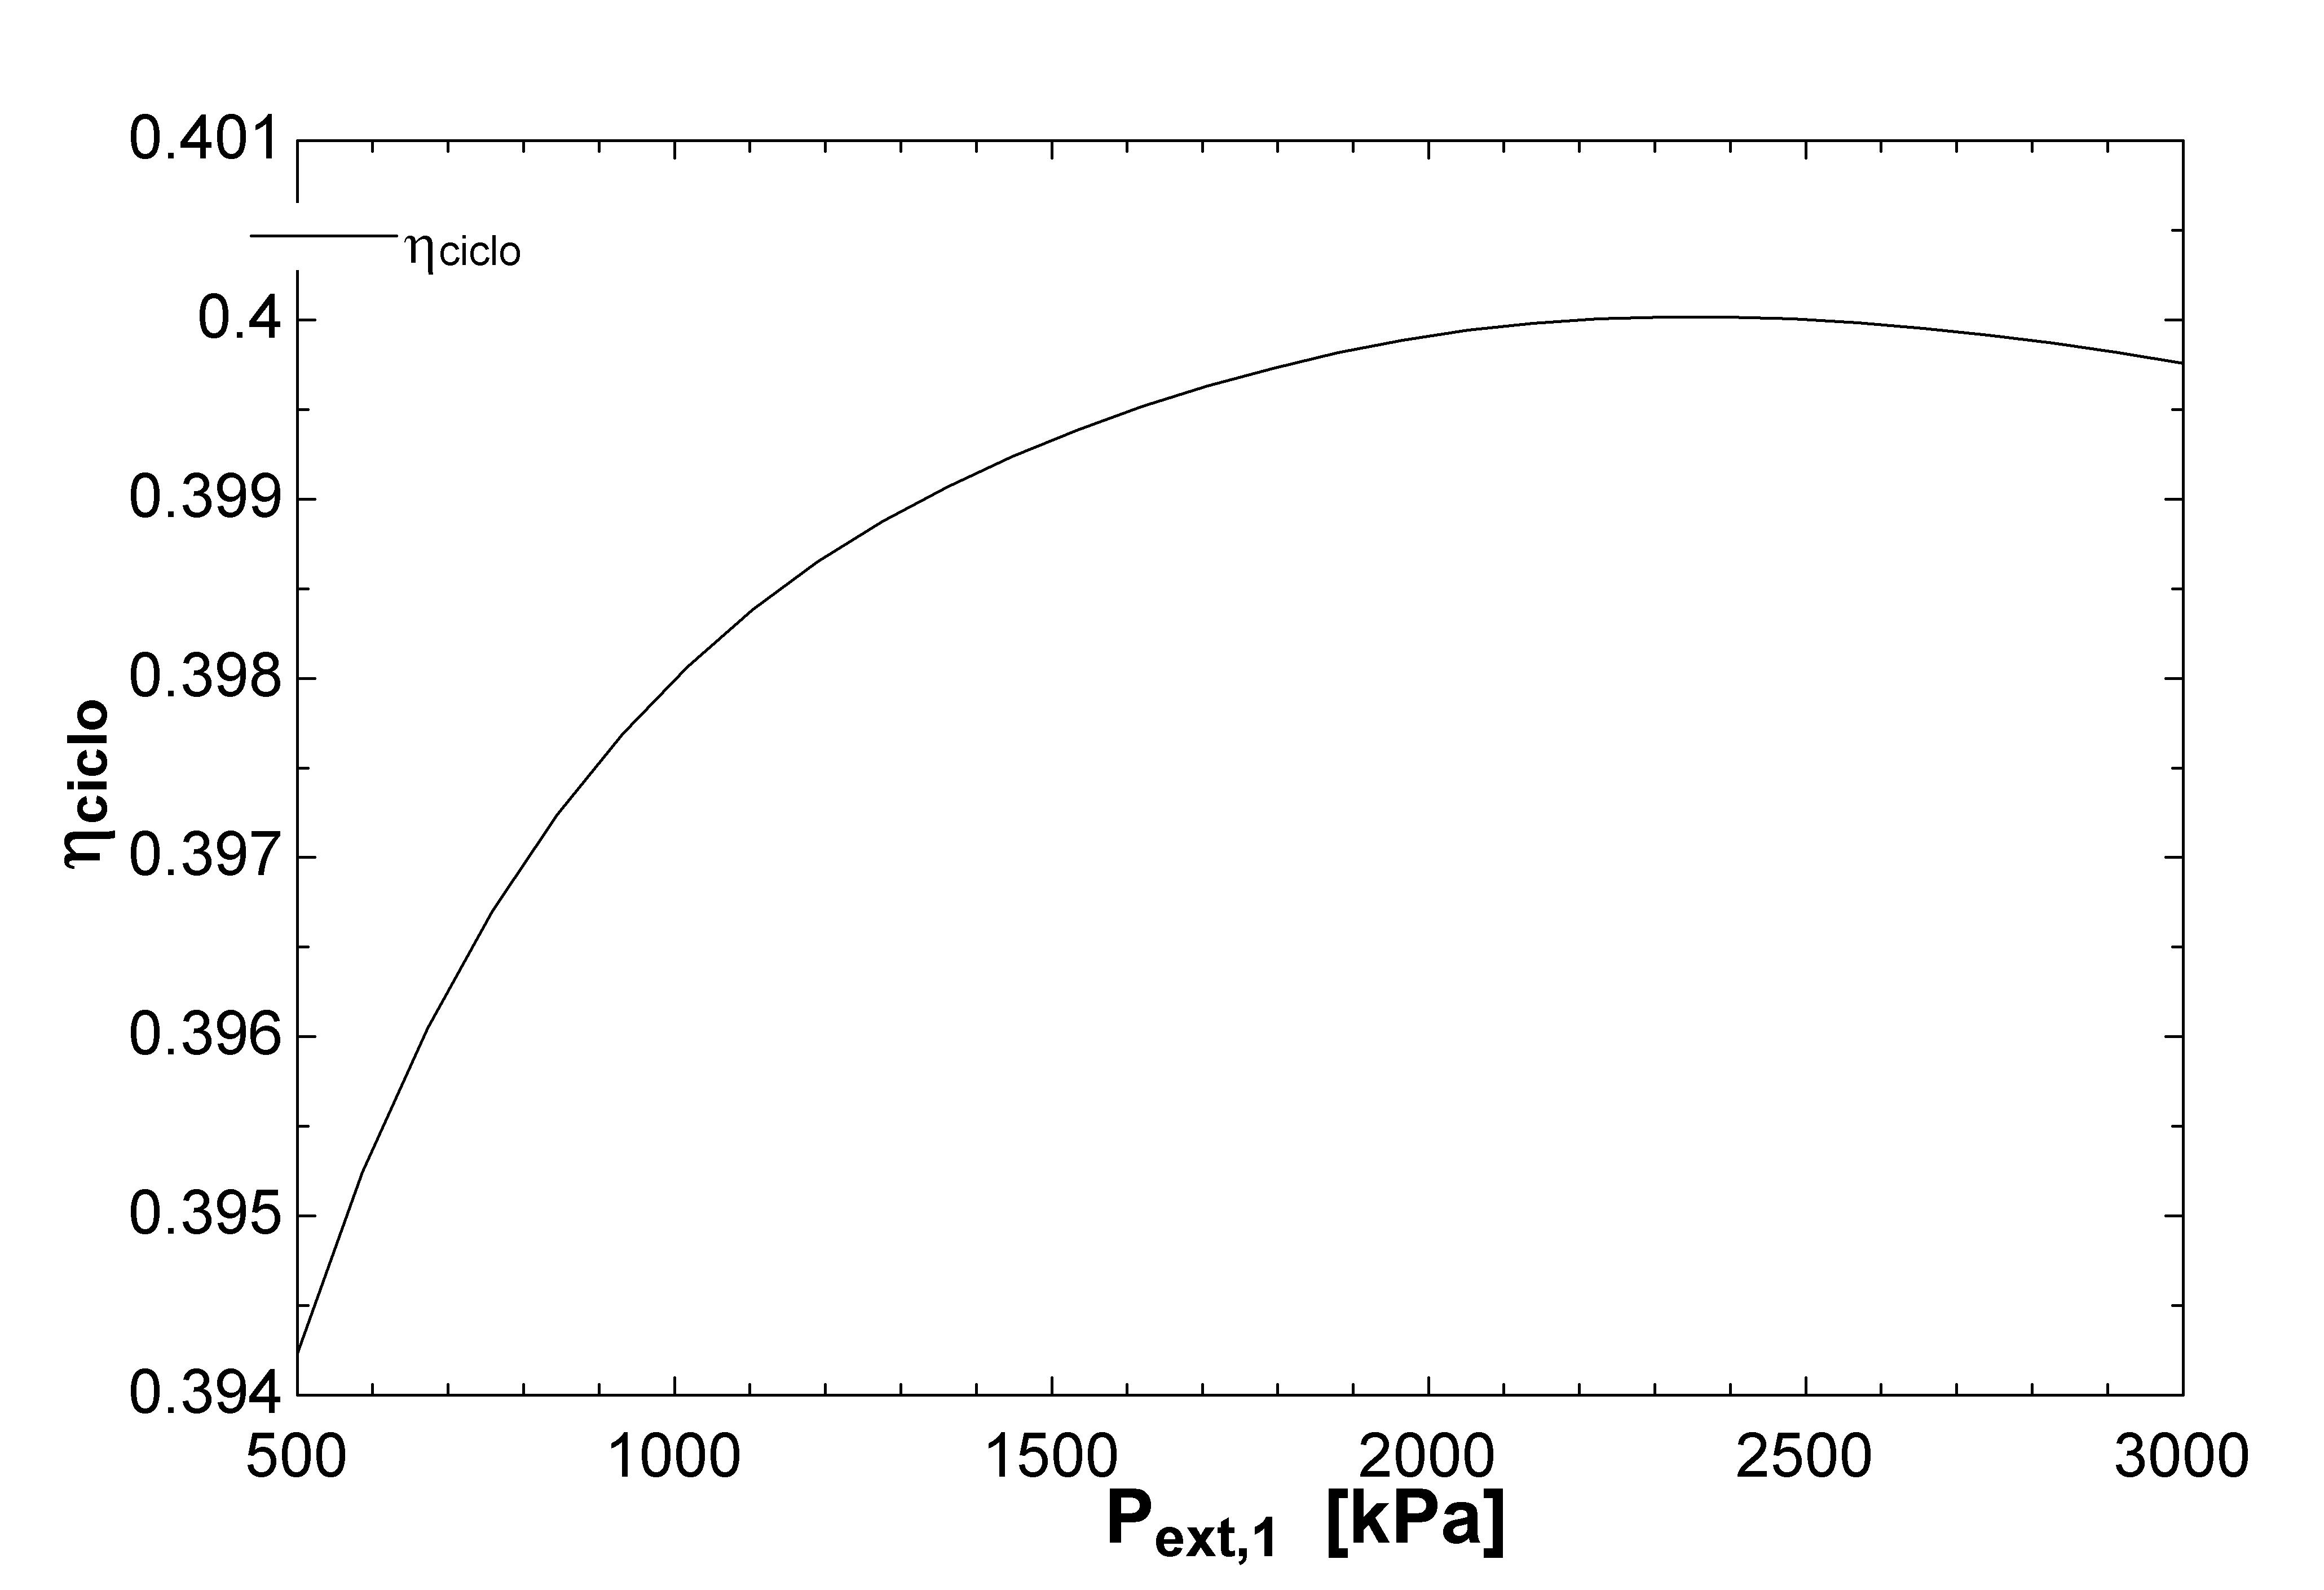
\includegraphics[width=5.0in,keepaspectratio]{Taller2_P2.jpg}}}
    \subsection*{Plot Window 2:\;Plot\;2}
    {\centerline{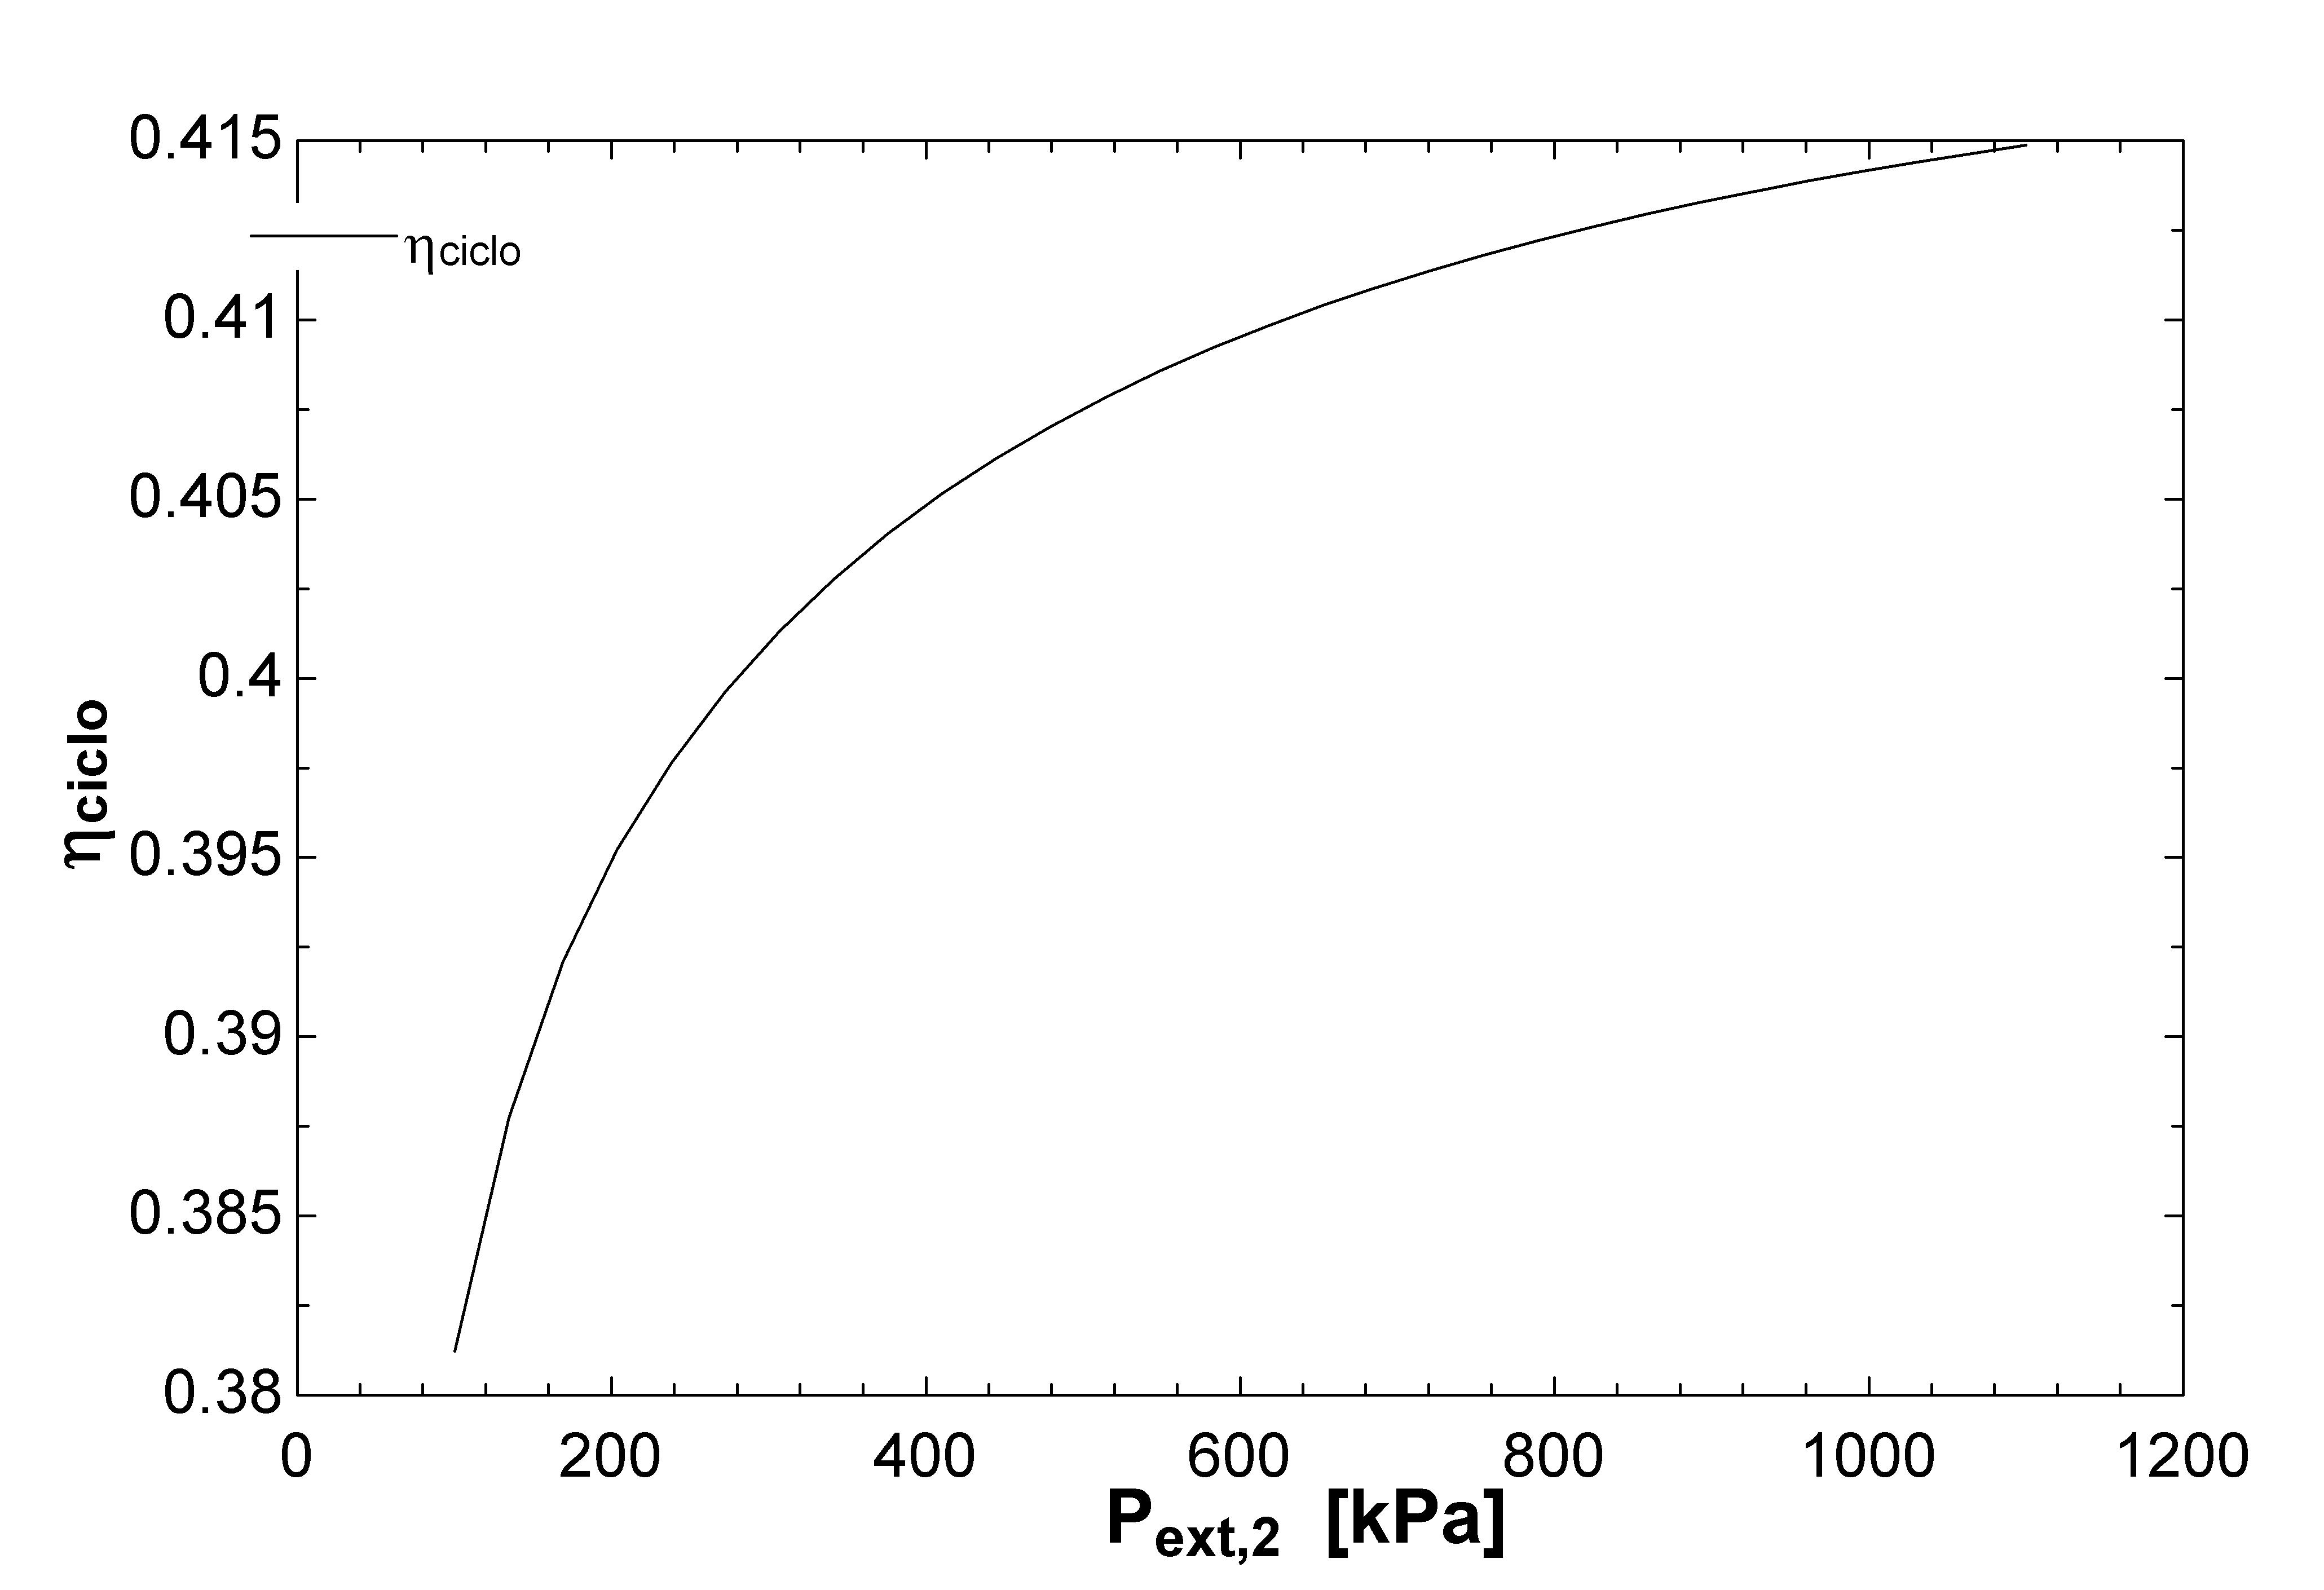
\includegraphics[width=5.0in,keepaspectratio]{Taller2_P3.jpg}}}
    \subsection*{Plot Window 3:\;Plot\;3}
    {\centerline{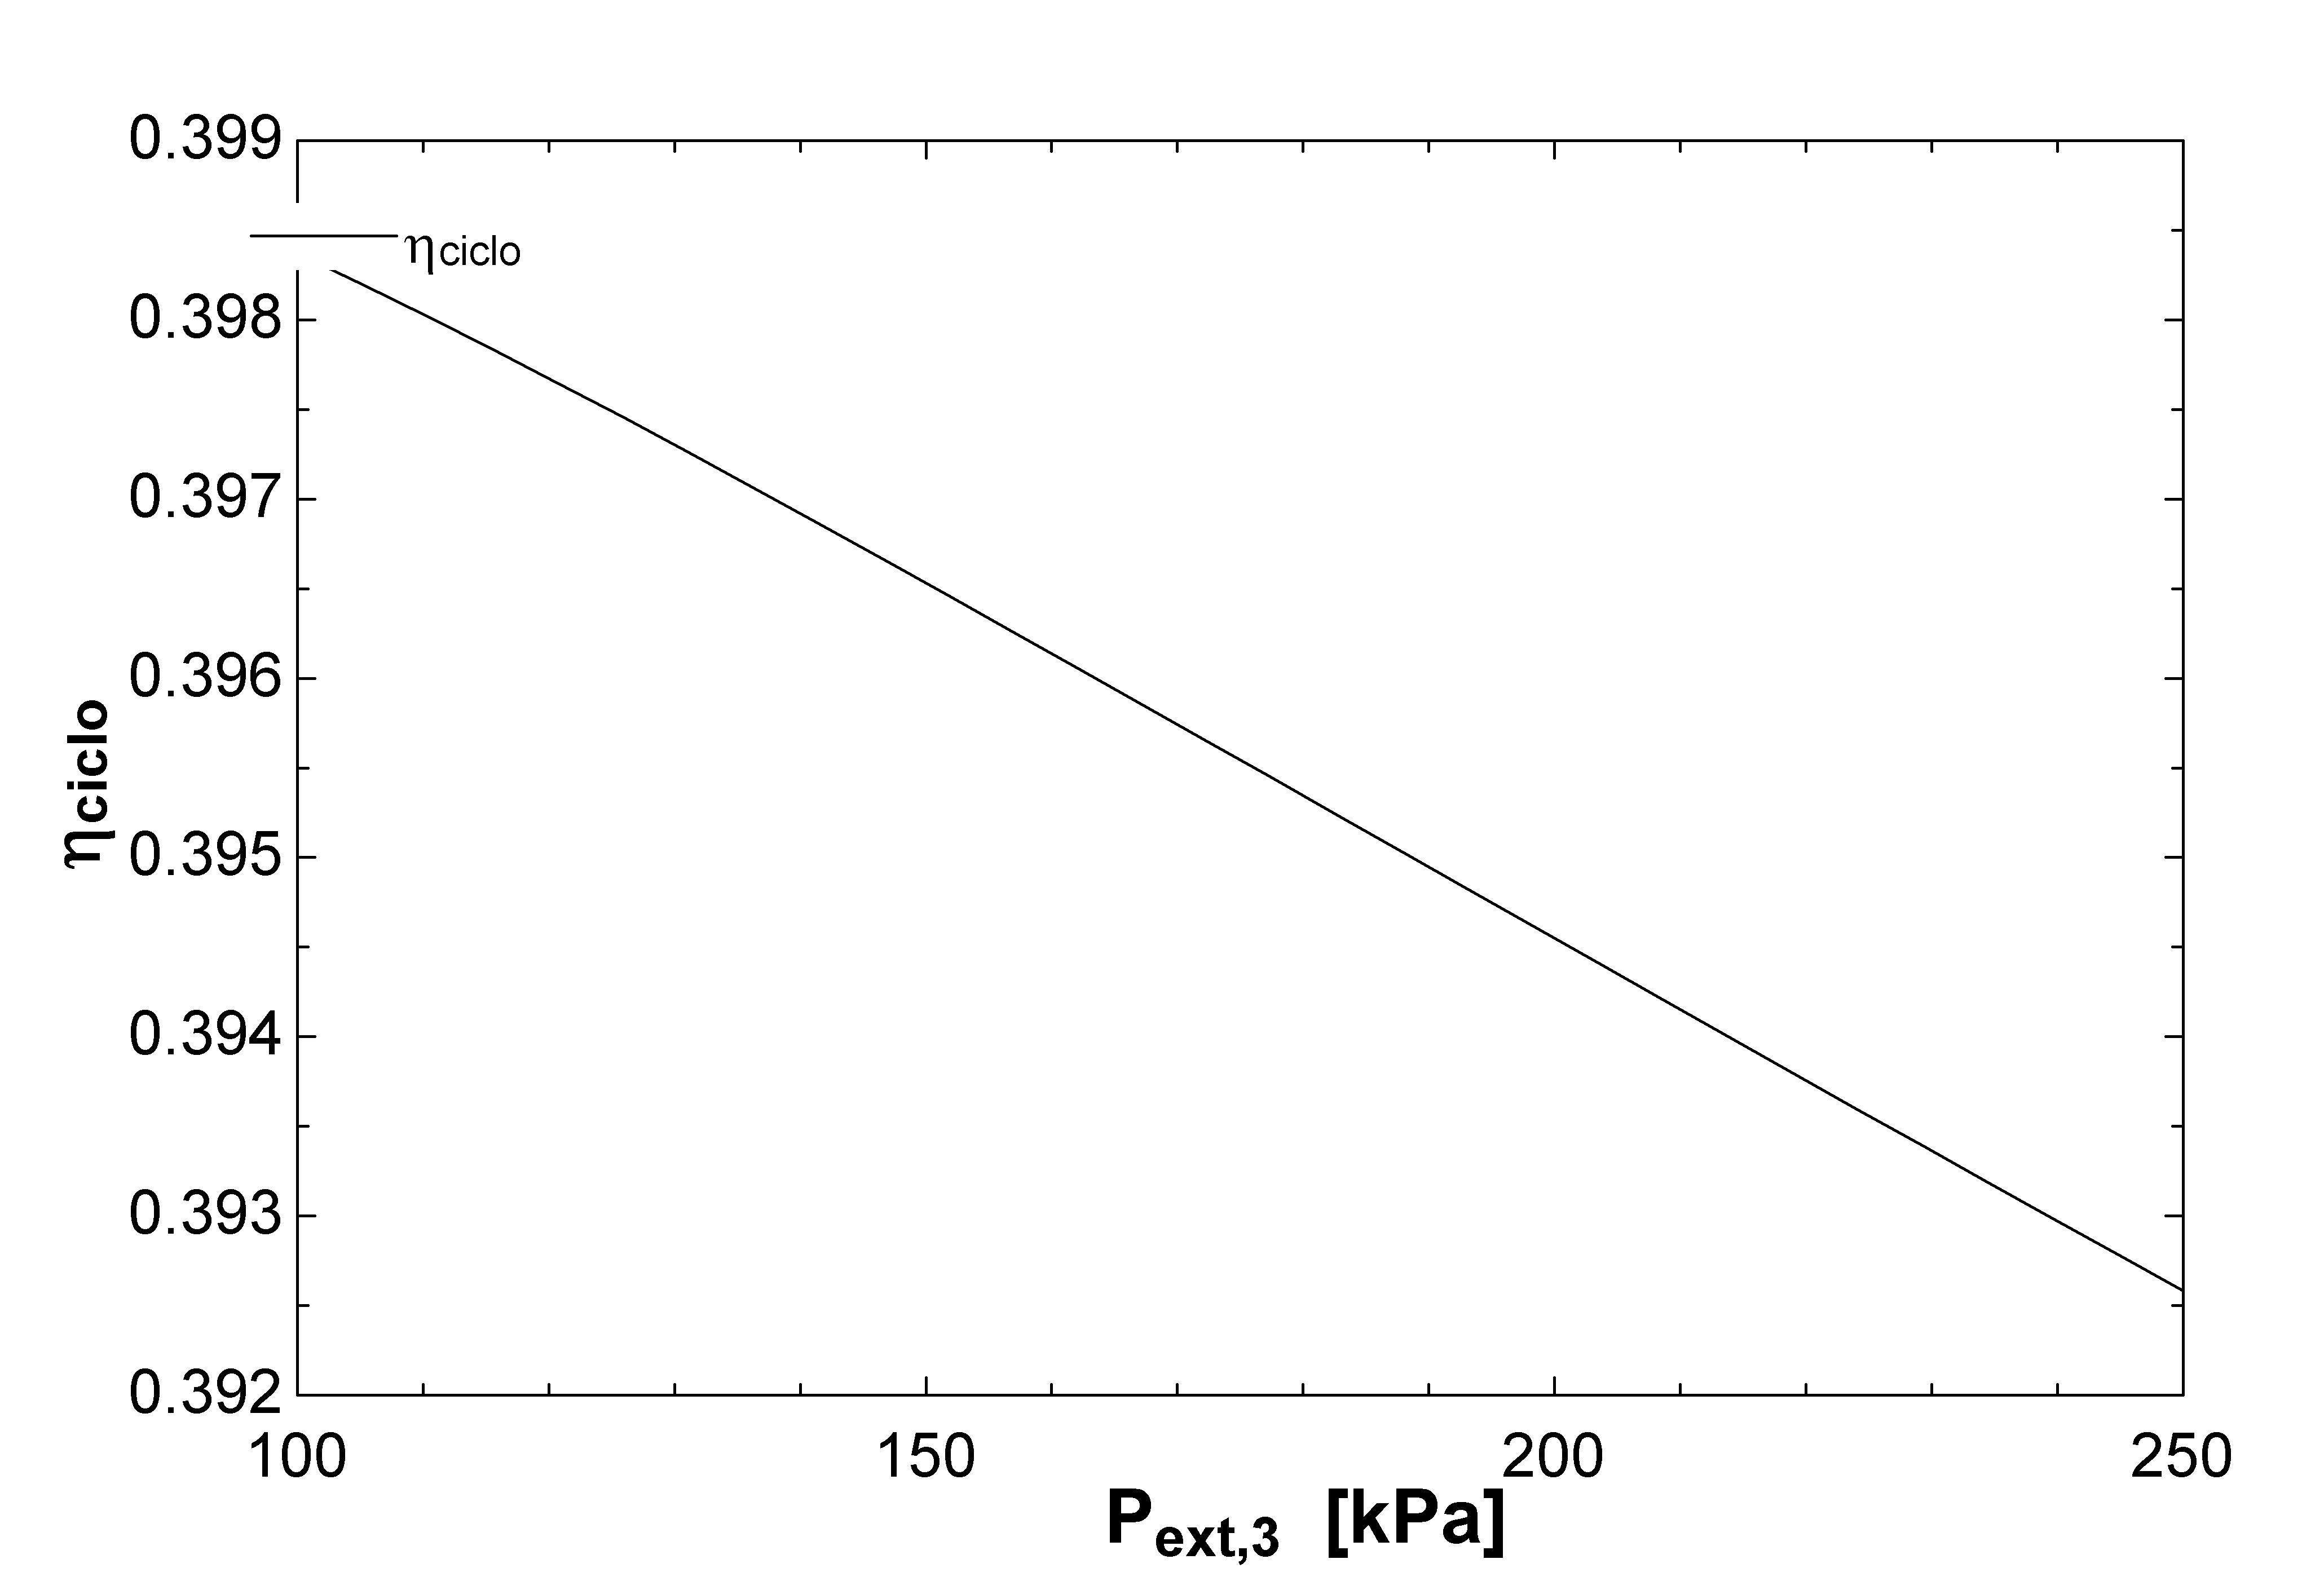
\includegraphics[width=5.0in,keepaspectratio]{Taller2_P4.jpg}}}   
    \begin{figure}[h!]
        \centering
        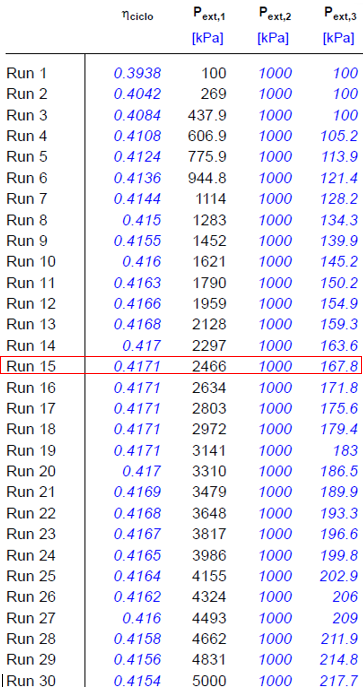
\includegraphics[width=0.4\linewidth]{Imagen2.png}
        \caption{Eficiencia vs variación de presión de extracción}
        \label{fig:etiqueta}
    \end{figure}
    \newpage
    Como resultado de la optimización con una eficiencia de ${\eta_{ciclo} =0.4171 \rm}$, se determinó que la configuración óptima de las presiones de extracción para el ciclo completo es:
   
    \begin{itemize}
        \item $P_{ext1} = 2466 \ \text{kPa}$
        \item $P_{ext2} = 1000 \ \text{kPa}$
        \item $P_{ext3} = 167.8 \ \text{kPa}$
    \end{itemize}
    \newpage
    \item A partir de lo estados definidos, se grafica en un diagrama T vs S, y se obtiene el resultado el siguiente gráfico:
    \subsection*{Plot Window 4:\;T-s:\;Water}
    {\centerline{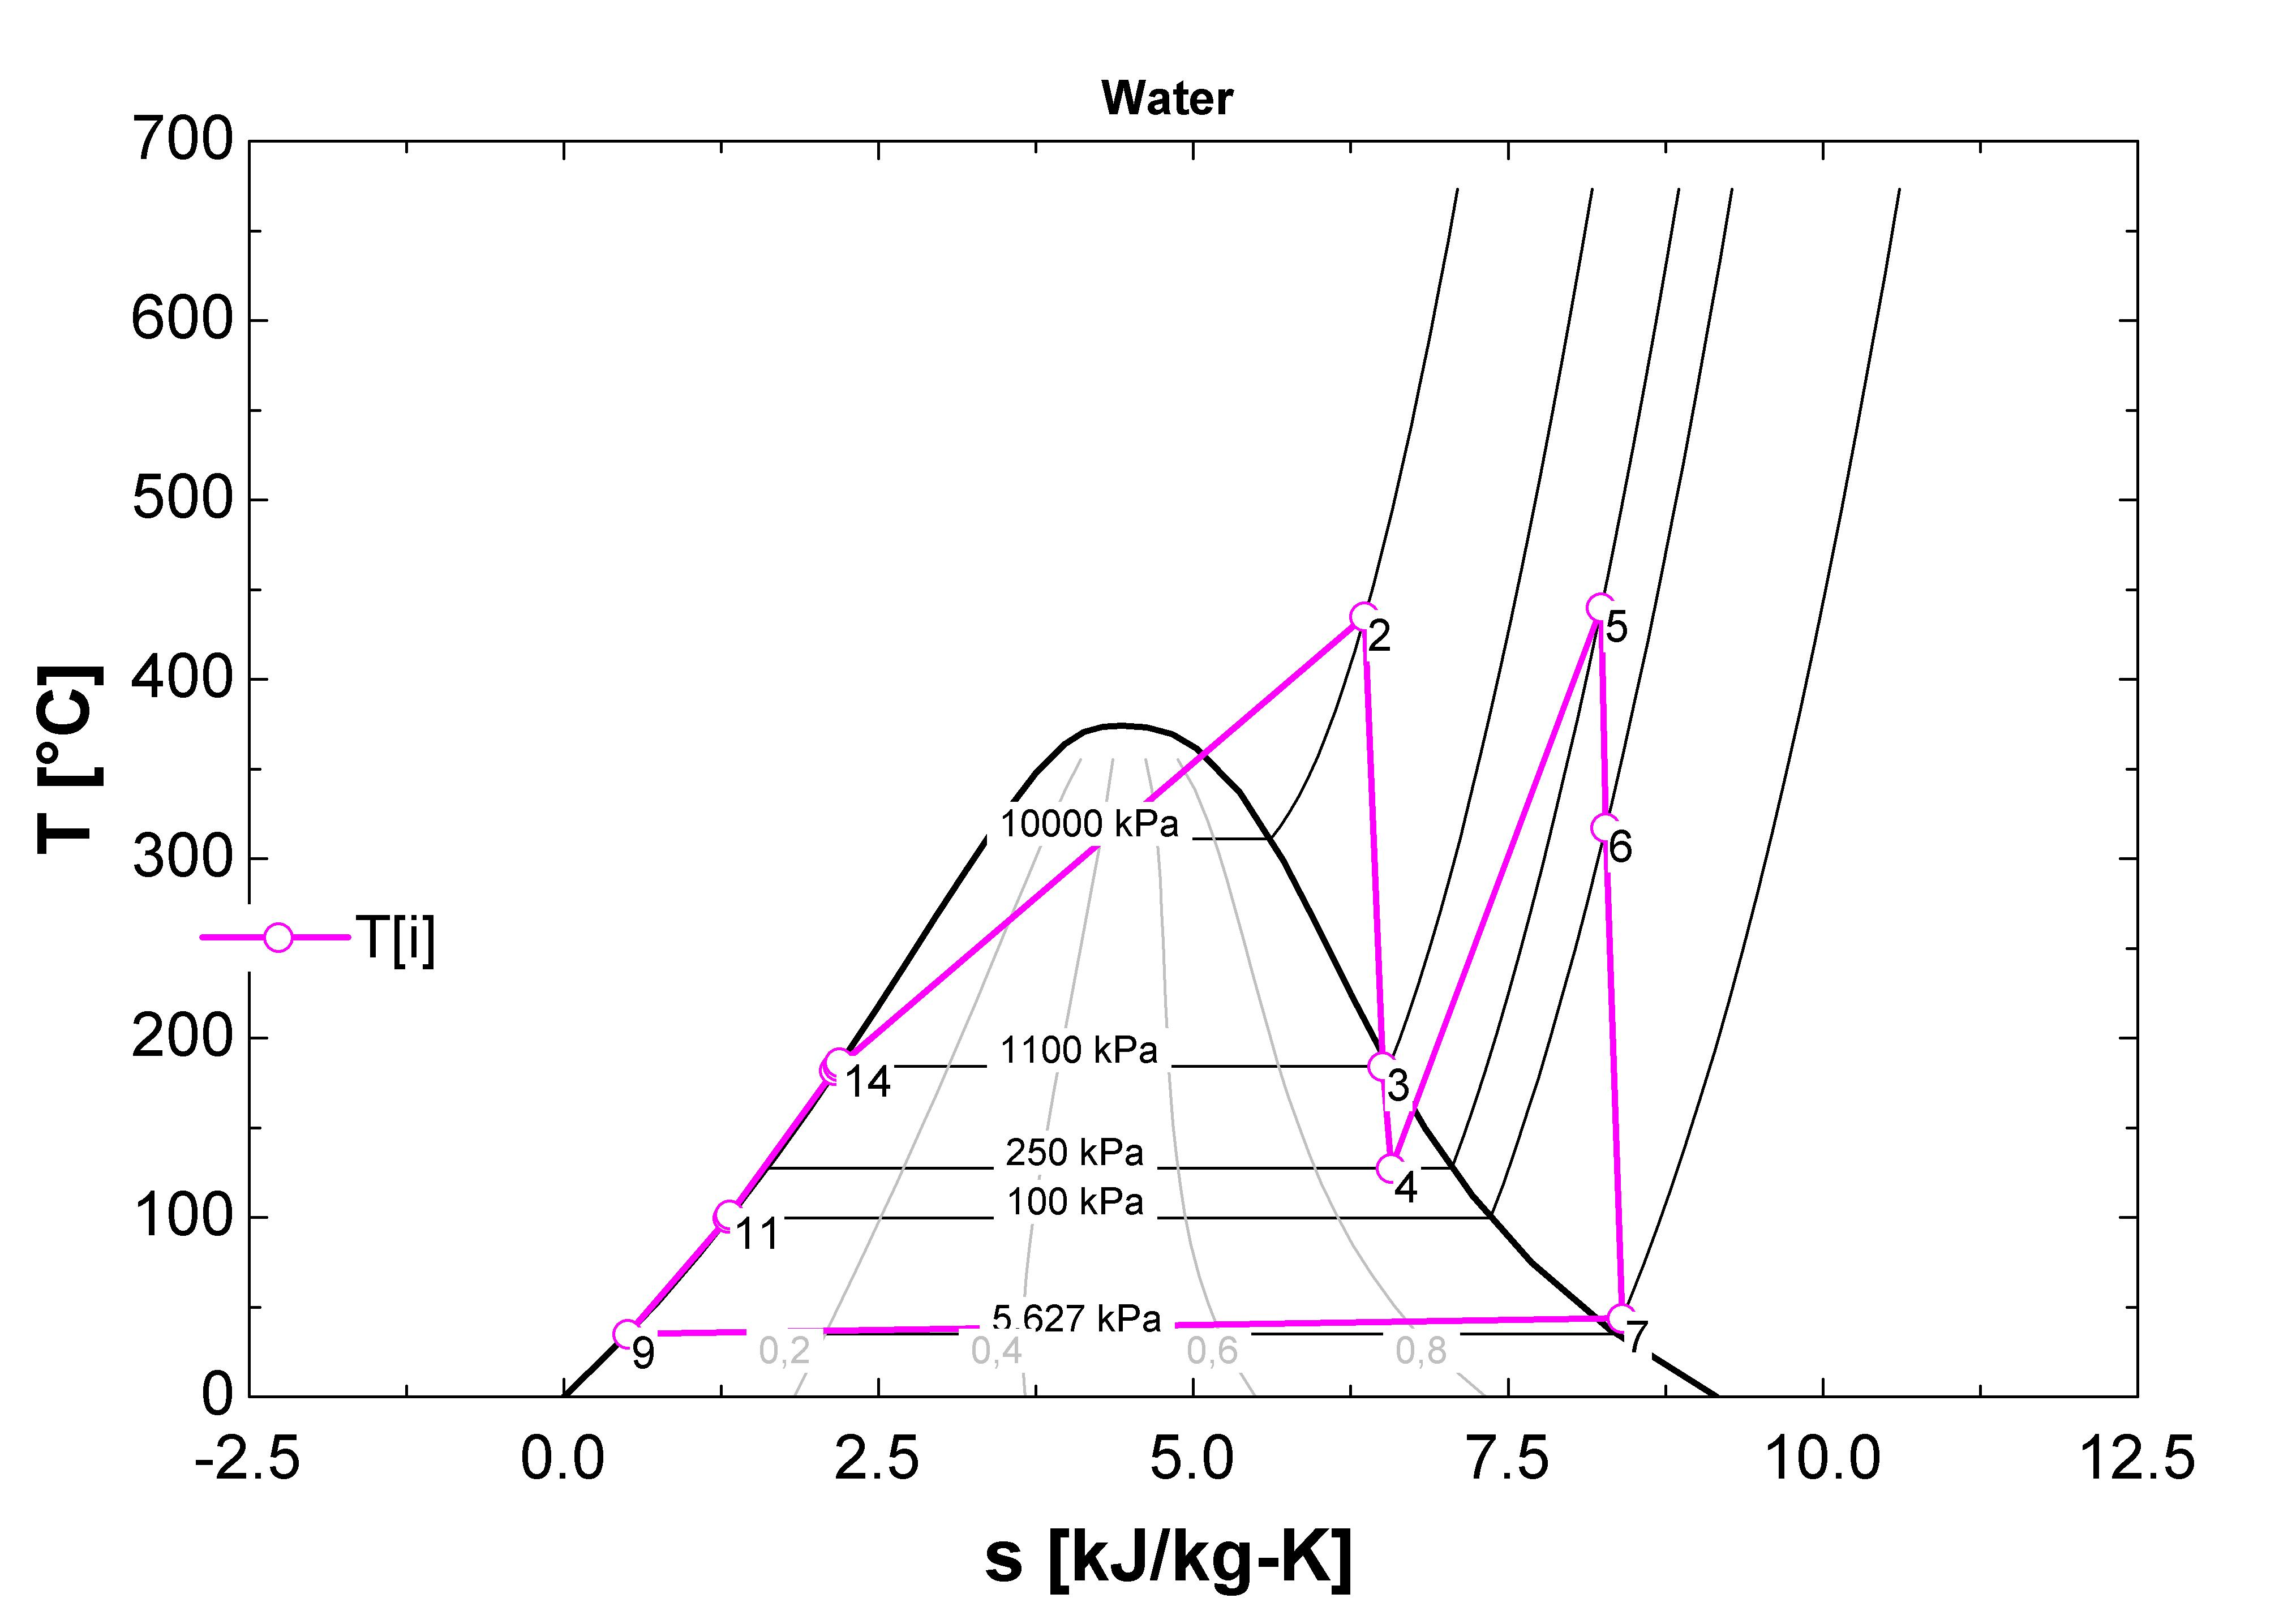
\includegraphics[width=5.0in,keepaspectratio]{Taller2_P1.jpg}}}
\end{enumerate}
\end{document}
